\documentclass[10pt,a4paper,twocolumn]{article}
\usepackage[T1]{fontenc}
\usepackage[utf8]{inputenc}
\usepackage{mathptmx}
\usepackage[margin=19mm,columnsep=6mm]{geometry}
\usepackage{amsmath,amssymb,graphicx,booktabs,tabularx}
\usepackage{microtype,xcolor,tikz}
\usepackage[numbers,sort&compress]{natbib}
\usepackage{balance}
\usetikzlibrary{arrows.meta,positioning}
\usepackage[font=small,labelfont=bf]{caption}
\usepackage[hidelinks]{hyperref}
\usepackage{url}
\urlstyle{same}
\setlength{\parindent}{1em}
\setlength{\parskip}{0pt}
\setlength{\textfloatsep}{10pt}
\setlength{\floatsep}{8pt}
\newcommand{\pending}{\textit{Pending}}
\newcommand{\code}[1]{\texttt{\detokenize{#1}}}
\title{Text-Prompted Plant Disease Lesion Segmentation\\with SAM 3 on PlantSeg}
% Author and affiliation are intentionally blank until supplied.
\author{}
\date{}
\hypersetup{pdftitle={Text-Prompted Plant Disease Lesion Segmentation with SAM 3 on PlantSeg}}
\raggedbottom
\begin{document}
\maketitle
\begin{abstract}
Plant disease lesion segmentation requires the localization of irregular symptoms in images with variable backgrounds, scales, and illumination. This paper describes a repository-grounded workflow for adapting Segment Anything Model 3 (SAM 3) to disease-conditioned lesion segmentation on PlantSeg. Disease names provide text prompts, while positive and negative queries supervise lesion localization and concept presence. The implementation combines pretrained visual and language representations with trainable fusion, localization, and segmentation components. The local PlantSeg v7 release contains 7,774 image--mask pairs across 115 disease categories and 34 host plants. A structural recheck confirms 21,580 orphan polygon annotations in the raw release; the existing annotation builder removes these records and produces 5,367 training, 846 validation, and 1,560 test images with polygon supervision. An earlier local audit additionally identifies polygon--mask disagreements and duplicate leakage, motivating a separate quality-controlled evaluation protocol. We document the implemented preprocessing, optimization settings, loss components, and validation metrics, and define the additional evaluation needed for final reporting. Model performance, learning curves, and prediction examples remain pending; this draft makes no empirical claim about segmentation accuracy or improvement over baselines.
\end{abstract}
\noindent\textbf{Keywords:} plant disease; lesion segmentation; SAM 3; text prompts; PlantSeg; transfer learning.

\section{Introduction}
Recognizing a disease label and delineating its visible symptoms are related but distinct tasks. A class label associates an image with a disease, whereas segmentation identifies the pixels occupied by annotated symptoms. Spatial delineation supports inspection of symptom distribution and can contribute to later image-based severity analysis. Field imagery complicates this task because symptoms may occupy small, disconnected areas, overlap with leaf veins, or resemble healthy tissue under changing illumination.

PlantSeg was introduced to support segmentation beyond controlled acquisition settings, providing disease masks together with host-plant and disease labels~\cite{plantseg}. The present project contains two local releases, v6 and v7, alongside a dataset audit and a training implementation. Their coexistence makes release selection and annotation interpretation essential: an image total alone does not specify the supervision used by a model.

SAM 3 extends promptable segmentation to concepts expressed through text or exemplars~\cite{sam3}. A disease phrase can therefore act as a condition for retrieving matching regions. This is attractive for PlantSeg because disease names already accompany each image. However, generic pretrained representations must still be evaluated against the visual ambiguity, fragmented lesions, and annotation conventions of this dataset.

This work documents an adaptation of the SAM 3 image model using the existing project implementation. It addresses three questions for subsequent experiments: (1) how accurately a pretrained model delineates lesions when given a disease prompt; (2) whether adaptation with frozen encoders improves that performance; and (3) how data-quality controls affect the conclusions. These questions remain open until training and test evaluation are completed.

The present contribution is a defined experimental workflow: a version-specific dataset characterization, an account of the implemented prompt and optimization strategy, and an evaluation plan that separates current validation behavior from publication metrics. The manuscript also identifies preparation steps still required to resolve known annotation problems. It does not introduce a new backbone or claim a measured improvement.

\section{Related Work}
\subsection{Dense segmentation}
U-Net couples a contracting path for contextual representation with an expanding path for spatial localization~\cite{unet}. DeepLabv3+ combines multiscale atrous context with a decoder that refines boundaries~\cite{deeplab}. They provide useful reference families for lesion segmentation, where both local boundaries and broader plant context matter. Neither model is implemented or evaluated in the current project; they are prospective comparison methods.

\subsection{Concept-conditioned segmentation}
SAM 3 accepts concept prompts and returns masks for matching instances; its presence mechanism separates concept recognition from localization~\cite{sam3}. This project uses its image pathway and disease-name prompts. It does not use video tracking or interactive point and box prompts. Adaptation tests a domain-specific use of an existing foundation model rather than an architectural modification.

\subsection{Plant disease benchmarks}
PlantSeg supplies disease-region supervision in visually diverse plant images~\cite{plantseg}. The local v7 copy corresponds to a versioned dataset release~\cite{plantsegv7}. Counts and partitions in this paper come from the local files rather than being inferred from the original paper. This distinction matters because local v6 and v7 differ in image availability, metadata, and effective supervision.

\section{Dataset and Annotation Audit}
\subsection{Evidence and scope}
The dataset description combines two evidence sources. A local audit dated 7 October 2026 reports full image and mask decoding, polygon comparisons, and duplicate screening~\cite{localaudit}. For this manuscript, metadata, file presence, annotation references, and the actual annotation-builder output were rechecked on 30 October 2026~\cite{snapshot}. This structural recheck did not repeat the pixel-level audit, duplicate search, or model inference. Historical audit findings are identified accordingly.

\begin{table}[t]
\centering\small
\caption{Local dataset releases. Disease counts refer to underlying labels; v6 metadata exposes only 114 IDs because of a soybean-rust labeling error. Coverage statistics are calculated from metadata.}
\label{tab:versions}
\begin{tabular}{lrr}\toprule
Property & v6 & v7\\\midrule
Image--mask pairs & 11,458 & 7,774\\
Training images & 7,916 & 5,367\\
Validation images & 1,247 & 846\\
Test images & 2,295 & 1,561\\
Host plants & 34 & 34\\
Disease categories & 115 & 115\\
Mean coverage (\%) & 21.4 & 21.4\\
Median coverage (\%) & 13.7 & 13.9\\\bottomrule
\end{tabular}
\end{table}

\subsection{Release selection and label representation}
The current script defaults to v7. Its 7,774 images are partitioned into 5,367 training, 846 validation, and 1,561 test samples (Table~\ref{tab:versions}). The previous audit reports that v7 retains a byte-identical subset of 7,774 v6 images and masks, with no split changes. Thus v6 and v7 must not be treated as independent datasets or used as separate training and test domains.

Each image has a same-stem PNG semantic mask and an associated metadata row. The mask value 0 denotes background, while nonzero values represent disease IDs offset by one. Each image has one labeled disease, potentially occupying multiple disconnected regions. The semantic mask therefore does not, by itself, define lesion instance identities. COCO polygon annotations supply the instance-style supervision consumed by the current training script.

Metadata provides disease names, plant names, class indices, split membership, and mask coverage. The v7 CSV requires UTF-8 BOM handling. The raw COCO files have empty category lists, so class names cannot be recovered from those lists alone. The training builder reconstructs categories from metadata. Its use of image-level metadata also overrides conflicting annotation category IDs; this is a labeling policy, not an independent confirmation of biological correctness.

\begin{figure*}[t]
\centering
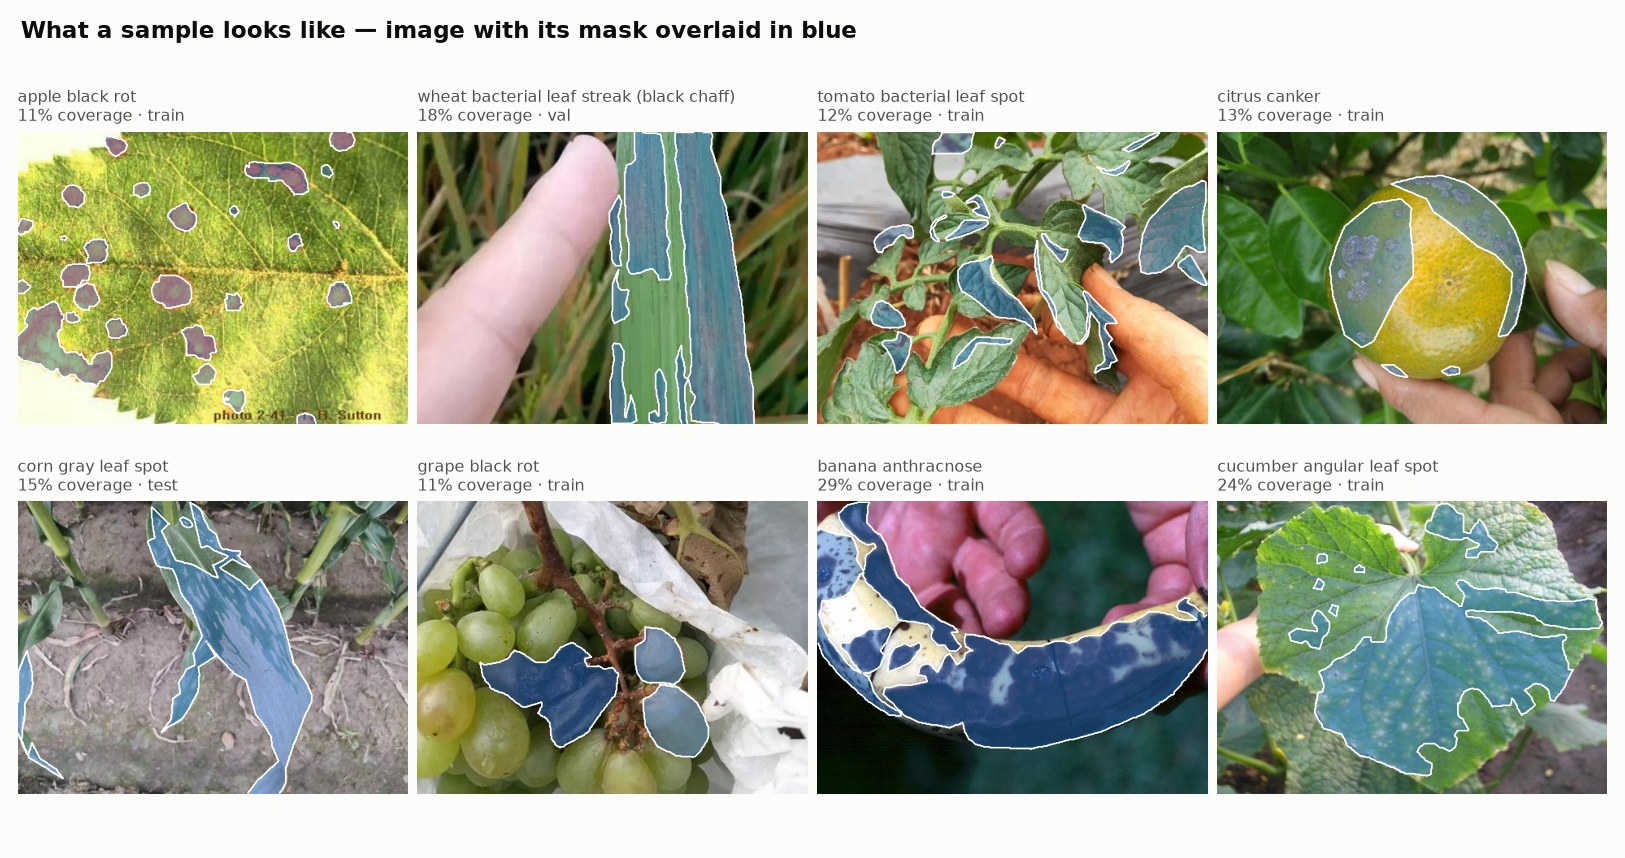
\includegraphics[width=\textwidth]{figures/dataset_samples.jpg}
\caption{PlantSeg examples from the existing local audit, with PNG ground-truth masks overlaid in blue. They illustrate fragmented spots, elongated symptoms, and extensive diseased regions. These are annotation examples, not model predictions. Source: local dataset audit~\cite{localaudit}.}
\label{fig:samples}
\end{figure*}

\subsection{Class and foreground imbalance}
The prior audit reports a long-tailed distribution: v7 class sizes range from 3 to 323 images, and 26 disease categories have fewer than 20 training images. Coffee black rot has no test image, while peach rust has no validation image. A class macro-average must therefore state the eligible class set and cannot silently assume support for every class in every partition.

Mean foreground coverage is approximately 21.4\%, with median coverage 13.9\%. The earlier pixel audit estimates that diseased pixels occupy 19.4\% of all v7 pixels when weighted by image size. Image-averaged coverage and pixel-weighted coverage are different statistics. Small regions can consequently contribute little to global pixel scores even when clinically or visually salient. Figure~\ref{fig:samples} illustrates the variety of annotation extent, including whole-region labels and individual spots.

\subsection{Raw and effective polygon supervision}
The structural recheck confirms that v7 retains 77,394 raw annotation records, of which 21,580 refer to image IDs absent from their split. The surviving records total 55,814. The project builder filters these orphan records, rejects polygons with invalid coordinate counts and boxes smaller than one pixel, normalizes numeric fields, and drops images with no remaining annotation.

\begin{table}[t]
\centering\small
\caption{Rechecked v7 annotation counts. ``Effective images'' are produced by the current builder before stochastic training transforms.}
\label{tab:effective}
\begin{tabular}{lrrr}\toprule
 & Train & Val. & Test\\\midrule
Raw images & 5,367 & 846 & 1,561\\
Raw polygons & 52,898 & 8,927 & 15,569\\
Orphan polygons & 14,647 & 2,467 & 4,466\\
Retained polygons & 38,251 & 6,460 & 11,103\\
Effective images & 5,367 & 846 & 1,560\\\bottomrule
\end{tabular}
\end{table}

The single excluded test image has a PNG mask but no polygon annotation. Therefore the script's effective polygon test set has 1,560 images, whereas a PNG-mask evaluation can retain all 1,561. Both the reference type and evaluated sample count must accompany any final score.

\subsection{Quality issues beyond structural filtering}
The earlier audit reports 180 v7 images whose polygons belong to another image, including 163 training samples. Structural filtering does not repair these shapes. The same audit identifies 107 validation and 183 test images with an exact or near duplicate in training. These are screened duplicate candidates based on image hashing and local review; the full duplicate analysis was not rerun for this paper.

Additional reported issues include conflicting disease labels and nine images with EXIF orientation flags. The inspected image loader converts opened images to RGB without an explicit EXIF transpose at that location. Orientation alignment must therefore be checked before a final experiment. The present training path also does not remove flagged duplicates or regenerate instances from PNG masks. These remain required preparation choices for the quality-controlled study described in Section~\ref{sec:protocol}.

\section{Method}
\subsection{Task formulation}
Given an RGB image $I$ and a disease phrase $t$, the model produces a set of masks, localization boxes, and confidence scores:
\begin{equation}
 f_\theta(I,t)=\{(M_j,b_j,s_j)\}_{j=1}^{Q}.
\end{equation}
For semantic lesion evaluation, accepted instance masks are combined into a foreground union. A positive prompt names the disease assigned to the image. A negative prompt names another annotated disease category and is supervised to return no lesion instance. This negative supervision assumes that the image-level annotation is exhaustive for the queried concept; unannotated co-occurring symptoms may violate that assumption.

Supplying the correct disease name defines \emph{disease-conditioned segmentation}. It does not establish automatic disease diagnosis. Querying all 115 names and selecting a disease is a separate evaluation task that the current validation routine does not implement.

\begin{figure}[t]
\centering
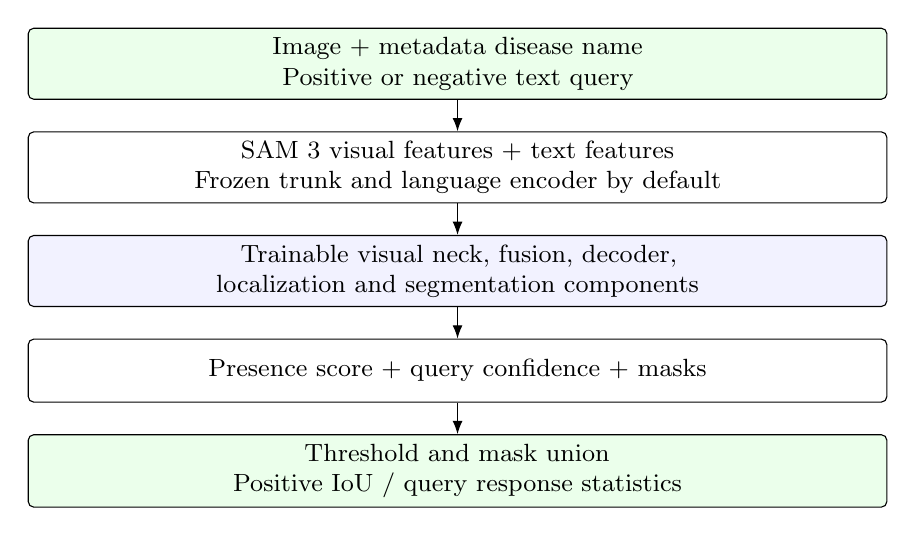
\begin{tikzpicture}[node distance=4mm,>=Latex,
 box/.style={draw,rounded corners=2pt,align=center,text width=0.88\columnwidth,minimum height=8mm,font=\small}]
\node[box,fill=green!8] (a) {Image + metadata disease name\\Positive or negative text query};
\node[box,below=of a] (b) {SAM 3 visual features + text features\\Frozen trunk and language encoder by default};
\node[box,below=of b,fill=blue!5] (c) {Trainable visual neck, fusion, decoder,\\localization and segmentation components};
\node[box,below=of c] (d) {Presence score + query confidence + masks};
\node[box,below=of d,fill=green!8] (e) {Threshold and mask union\\Positive IoU / query response statistics};
\draw[->] (a)--(b);\draw[->] (b)--(c);\draw[->] (c)--(d);\draw[->] (d)--(e);
\end{tikzpicture}
\caption{Implemented image-model workflow. The diagram depicts the default adaptation scope; full fine-tuning is an optional script setting.}
\label{fig:pipeline}
\end{figure}

\subsection{Backbone and adaptation scope}
The implementation builds the SAM 3 image model with segmentation enabled and pretrained weights supplied locally or retrieved through the model builder. Its visual trunk uses a vision transformer; language features represent the supplied phrases. Fusion and decoding produce concept-conditioned localization and segmentation outputs. Figure~\ref{fig:pipeline} summarizes this path.

The default \code{heads} scope freezes the visual transformer trunk and the language backbone. Other components, including the visual neck, remain trainable. Consequently the scope name should not be interpreted as training only a final prediction layer. The alternative \code{full} scope enables optimization of all parameters. No adaptation-scope comparison has yet been measured.

With frozen language features, the script encodes the fixed disease vocabulary once, caches the resulting tensors, and removes the language module from the active model. This makes training dependent on that fixed prompt vocabulary. Experiments using alternative prompt wording require recomputing compatible features. Adaptation checkpoints save trainable parameters rather than a complete standalone model, so reproducing inference also requires the matching pretrained base and adaptation settings.

\subsection{Prompt construction and sampling}
Prompt text is the lowercased metadata disease name; the plant field is retained for negative sampling. During training the positive category is retained with probability 0.7. The default uses one prompt per image, so a selected example normally supplies either its positive disease or a negative disease, rather than both simultaneously.

For remaining prompt slots, the sampler first requests up to $\lceil K/2\rceil$ absent diseases from the same plant and fills the remainder from other plants, where $K$ is the number of negative slots. With the one-prompt default, the negative is from the same plant whenever such a category is available. This creates a challenging contrast between diseases that share host appearance. Increasing the prompt count changes both query composition and memory demand.

Validation always includes the positive disease and, by default, two negative categories. Negative selection uses an image-index-seeded random generator, providing repeatable choices within the same dataset ordering. The number of returned negatives can depend on available categories. A run must record its resulting prompt set and negative-query count for interpretation of false-positive rates.

\subsection{Image transforms}
The model path uses a 1,008-pixel reference resolution. Training decodes segmentations, applies a random horizontal flip and square scale jitter generated from a 480-pixel minimum, pads to $1{,}008\times1{,}008$, converts to tensors, and normalizes each channel with mean and standard deviation 0.5. Filters remove zero-area targets and restrict training examples to at most 200 output objects per query. Validation uses a deterministic square resize to the reference resolution and the same normalization.

Resizing is shared between image and annotation geometry, but square resizing changes aspect ratio. Padding and low-resolution mask output also affect how an IoU score should be interpreted. Final PNG evaluation should explicitly map outputs to the original, orientation-corrected coordinate frame. That evaluation is an addition to the current validation helper.

\subsection{Matching and supervision}
The criterion uses binary Hungarian matching with class, box-distance, and generalized-IoU costs weighted 2, 5, and 2. An additional one-to-many matcher uses $\alpha=0.3$, threshold 0.4, and top-$k=4$, with an overall weight of 2. The loss wrapper combines localization, classification, presence, instance-mask, and semantic-region supervision.

At the component level, configured weights are
\begin{align}
\mathcal L_{\mathrm{loc}} &=5\mathcal L_{\mathrm{box}}+2\mathcal L_{\mathrm{GIoU}},\\
\mathcal L_{\mathrm{concept}} &=20\mathcal L_{\mathrm{cls}}+20\mathcal L_{\mathrm{pres}},\\
\mathcal L_{\mathrm{inst}} &=200\mathcal L_{\mathrm{mask}}+10\mathcal L_{\mathrm{Dice}},\\
\mathcal L_{\mathrm{sem}} &=20\mathcal L_{\mathrm{sem\mbox{-}focal}}
                         +30\mathcal L_{\mathrm{sem\mbox{-}Dice}}.
\end{align}
These expressions summarize configured component weights; the upstream wrapper also handles matching branches, auxiliary outputs, and normalization. Instance-mask focal settings use $\alpha=0.25$, $\gamma=2$, while the semantic focal settings use $\alpha=0.6$, $\gamma=2$. The semantic criterion disables its separate presence-loss term. Instance-mask auxiliary losses are disabled. This is a composite supervised adaptation objective, not a single binary-mask loss.

\subsection{Optimization and memory management}
Table~\ref{tab:settings} gives the current command-line defaults, not a completed experiment's configuration. AdamW applies weight decay to multidimensional parameters and excludes biases and one-dimensional parameters. An inverse-square-root schedule includes warm-up and cooldown. The script evaluates each epoch, selects the best checkpoint by validation IoU, and writes a latest checkpoint.

\begin{table}[t]
\centering\small
\caption{Implemented default configuration. Actual run settings and hardware remain to be recorded.}
\label{tab:settings}
\begin{tabular}{lr}\toprule
Setting & Value\\\midrule
Adaptation scope & Frozen trunk and text\\
Epochs & 20\\
Images per training batch & 1\\
Gradient accumulation & 8\\
Training prompts per image & 1\\
Positive-prompt probability & 0.7\\
Validation negative prompts & 2\\
Transformer/head learning rate & $8\times10^{-5}$\\
Visual-component learning rate & $2.5\times10^{-5}$\\
Language learning rate (full scope) & $5\times10^{-6}$\\
Weight decay / gradient clip norm & 0.1 / 0.1\\
Requested warm-up steps & 100\\
Cooldown fraction & 0.1\\
Score threshold & 0.5\\
Random seed / data workers & 0 / 4\\\bottomrule
\end{tabular}
\end{table}

The nominal effective batch is eight images per optimizer update. The implemented loop updates only on complete accumulation groups; it does not flush a partial group at epoch end. With the unfiltered 5,367-image training set and batch size one, this gives 670 scheduled updates per epoch, subject to runtime filtering and skipped nonfinite losses. Warm-up is capped at one quarter of scheduled steps, and cooldown is at least one step.

Mixed precision is selected from GPU capability, with optional reduced-precision storage for frozen modules. The code includes a differentiable fallback for a fused visual MLP and convolution-layout handling for older GPUs. These are implementation choices whose numerical stability and memory use require measurement on the eventual training machine; they are not evidence that a complete run fits a particular device.

\section{Experimental Protocol}
\label{sec:protocol}
\subsection{Current validation metrics}
For query $q$ and instance $j$, the existing helper multiplies the sigmoid query logit by the sigmoid concept-presence logit:
\begin{equation}
 s_{qj}=\sigma(z_{qj})\sigma(p_q).
\end{equation}
It accepts instances with $s_{qj}>0.5$, thresholds mask logits at zero, and takes their union:
\begin{equation}
 \widehat G_q=\bigcup_{j:s_{qj}>0.5}\{x:\ell_{qj}(x)>0\}.
\end{equation}
Ground-truth instance masks are area-resampled to the output-mask size and binarized at 0.5 before union. The resulting IoU is averaged across positive queries. It is a polygon-derived, output-resolution score, not native-resolution PNG-mask IoU.

The logged \code{val_recall} is the fraction of positive queries for which at least one instance survives the score threshold. It does not require spatial overlap and is therefore a positive-query response rate rather than lesion detection recall. Similarly, \code{val_false_positive} is the fraction of sampled negative queries with any accepted instance. It is a query-level false-alarm rate, not a pixel false-positive rate. These distinctions must remain explicit when importing training logs into the results section.

\subsection{Final segmentation metrics to add}
The primary final evaluation should use the union of predicted disease regions against the binary PNG reference $G=\{x:Y(x)>0\}$ in the original aligned image frame. With pixel counts TP, FP, and FN, define
\begin{align}
\mathrm{IoU}&=\frac{\mathrm{TP}}{\mathrm{TP}+\mathrm{FP}+\mathrm{FN}},\\
\mathrm{Dice}&=\frac{2\mathrm{TP}}{2\mathrm{TP}+\mathrm{FP}+\mathrm{FN}}.
\end{align}
Pixel precision and recall are $\mathrm{TP}/(\mathrm{TP}+\mathrm{FP})$ and $\mathrm{TP}/(\mathrm{TP}+\mathrm{FN})$. For a nonempty reference and empty prediction, IoU, Dice, and recall are zero; prediction precision is undefined and should be reported as such. Empty references and absent disease classes require an explicit policy rather than an implicit smoothing convention.

Report image-mean IoU and Dice, pooled foreground IoU, and a disease-macro score. For class $c$ with $n_c$ eligible test images,
\begin{equation}
 \mathrm{mIoU}_{\mathrm{disease}}=
 \frac{1}{|\mathcal C_*|}\sum_{c\in\mathcal C_*}
 \frac{1}{n_c}\sum_{i:y_i=c}\mathrm{IoU}_i,
\end{equation}
where $\mathcal C_*$ contains classes with test support. This is an average of image scores within disease, then across diseases. It differs from averaging classwise pooled confusion matrices and from averaging disease and background semantic IoUs.

Dice, precision, disease-macro aggregation, uncertainty estimates, and native-resolution PNG evaluation are not currently produced by the helper. Instance AP may be added only after polygon quality and instance definitions have been resolved. A mask connected component is an operational pseudo-instance and should not be represented as an expert-verified lesion identity.

\subsection{Data preparation and split policy}
Two protocols should be distinguished. The \emph{existing split} protocol preserves the local partition and reports its known duplicate risk. The \emph{quality-controlled} protocol verifies orientation, resolves flagged polygon mismatches, and removes training images belonging to validation or test duplicate clusters. If a cluster spans validation and test, it must also be assigned to one evaluation partition or explicitly excluded. A saved manifest must define these choices, final class support, and exclusions.

The currently available duplicate screening can initialize this process, but its threshold-based clusters need review before a final manifest is frozen. No corrected manifest has been generated by this report. Dataset tables describe the available files and current builder, not an already cleaned benchmark.

Hyperparameters, stopping criteria, and thresholds should be selected on validation only. The test partition should be evaluated after those decisions are fixed. Include all 1,561 v7 test PNG pairs for semantic evaluation unless the chosen quality policy explicitly removes samples. Document every exclusion, including any difference from the builder's 1,560 polygon-supported images.

\subsection{Comparisons and ablations}
The primary comparison is pretrained SAM 3 without adaptation versus the default frozen-encoder adaptation, using identical disease prompts, preprocessing, and scoring. A full-adaptation configuration can test whether updating representations adds value when resources permit. Further controlled ablations can vary positive-only versus negative-query training, same-plant versus other-plant negatives, and original versus quality-controlled supervision.

U-Net and DeepLabv3+ are optional future semantic baselines. Their output task and use of disease labels must be specified to make a comparison interpretable. A generic lesion model that receives no disease name has a different input contract from a model given the correct disease phrase. None of these prospective baselines or ablations is claimed as completed.

Use multiple training seeds if feasible and report their mean and variation. Resampling uncertainty should respect duplicate clusters rather than treating near-identical images as independent observations. Also analyze small-coverage images and rare diseases separately. Prompted localization is not a substitute for a disease-classification experiment, so conclusions should remain conditional on the supplied prompt.

\subsection{Reproducibility records}
A final run should preserve the pretrained checkpoint identifier and hash, source revision, resolved arguments, dataset manifest, prompt vocabulary, seed, software versions, GPU model, optimizer updates, and checkpoint-selection rule. Record peak allocated GPU memory and latency with input size, precision, batch size, and synchronization policy. All these runtime measurements remain pending.

The report evidence snapshot records source and dataset hashes and the vendored SAM 3 revision. The existing script produces JSONL training logs and adaptation checkpoints. Resuming additionally requires a compatible base model and optimizer state. The main entry point currently runs training and validation; a standalone test evaluator must be supplied for the final protocol above.

\section{Results}
\label{sec:results}
\subsection{Verified preparation findings}
The structural inspection establishes dataset availability and annotation-builder behavior. It confirms the release totals in Table~\ref{tab:versions}, orphan-annotation removal in Table~\ref{tab:effective}, and the distinction between raw image--mask pairs and effective polygon supervision. These are data-preparation findings. They do not measure segmentation quality, convergence, generalization, or hardware feasibility.

The builder also reports 67 training and 40 test v7 annotations whose category differs from the image metadata. It rewrites those categories to the metadata class while preserving polygon geometry. This check reinforces why successful COCO construction alone is insufficient to demonstrate annotation correctness.

\subsection{Quantitative performance}
Model results will be inserted after training and evaluation. Table~\ref{tab:results} reserves the primary comparison. Every pending entry means that no verified measurement is available; it does not represent zero performance. All final values must share the same reference masks, split manifest, and prompt assumptions.

\begin{table}[!ht]
\centering\small
\caption{Primary performance table to complete using original-frame PNG masks. IoU and Dice are image means; Macro is disease-macro IoU. Additional pixel and negative-query statistics should accompany the final table.}
\label{tab:results}
\setlength{\tabcolsep}{3pt}
\begin{tabularx}{\columnwidth}{Xccc}\toprule
Configuration & IoU & Dice & Macro\\\midrule
SAM 3 pretrained & \pending & \pending & \pending\\
Frozen-encoder adaptation & \pending & \pending & \pending\\
Full adaptation (optional) & \pending & \pending & \pending\\\bottomrule
\end{tabularx}
\end{table}

\subsection{Learning behavior and efficiency}
Training and validation curves will be added from run logs with explicit epoch or update axes. The selected checkpoint, stopping epoch, skipped nonfinite batches, and validation criterion must accompany them. A change in validation IoU should not be interpreted as a native-resolution test improvement without the corresponding test evaluation.

\begin{table}[!ht]
\centering\small
\caption{Runtime and training record to complete for the selected adapted model.}
\label{tab:runtime}
\begin{tabular}{lr}\toprule
Record & Measurement\\\midrule
GPU / software environment & \pending\\
Final data-manifest identifier & \pending\\
Training scope / actual precision & \pending\\
Trainable parameter count & \pending\\
Selected epoch / optimizer updates & \pending\\
Training duration & \pending\\
Peak GPU memory & \pending\\
Inference latency per image and prompt & \pending\\\bottomrule
\end{tabular}
\end{table}

\subsection{Qualitative analysis}
Prediction panels will compare input images, PNG references, pretrained outputs, and adapted outputs for identical disease prompts. Include successful cases and errors involving tiny lesions, extensive symptoms, clutter, and ambiguous tissue. Negative-query examples should expose spurious responses. Annotated dataset examples in Fig.~\ref{fig:samples} cannot replace these prediction panels.

\begin{figure}[t]
\centering
\fbox{\parbox[c][27mm][c]{0.91\columnwidth}{\centering\small
Prediction panels pending\\[3pt]
Input image $\mid$ PNG reference\\
Pretrained mask $\mid$ Adapted mask\\[3pt]
Add disease prompt, confidence rule, and per-image IoU.}}
\caption{Reserved location for actual model predictions. No synthetic prediction or unmeasured score is displayed.}
\label{fig:predictions}
\end{figure}

\subsection{Ablation and error analysis}
After the primary run, report the effect of negative-query sampling and adaptation scope using a fixed split and validation procedure. Compare the original and quality-controlled protocols with their own denominators. Discuss rare-class errors and the sensitivity of small lesions to mask resolution. Statistical or causal claims about any design choice remain deferred until the corresponding controlled comparisons are available.

\section{Discussion and Limitations}
The current workflow links disease vocabulary to localized regions and reuses pretrained representations while restricting default encoder updates. This provides a concrete adaptation strategy to evaluate, but its benefit over unadapted inference is still unknown. The availability of loss functions, memory-oriented code paths, and checkpoint handling does not demonstrate successful optimization.

Annotation choice is a central limitation. The training script learns from polygons, whereas the earlier audit recommends PNG masks as a more reliable semantic reference for flagged samples. Relabeling a polygon from metadata leaves incorrect geometry unchanged. Excluding faulty records or regenerating pseudo-instances can reduce this inconsistency, but either action changes the supervision and needs an explicit manifest and ablation.

Duplicate leakage and limited rare-class support constrain generalization claims. A high aggregate score could reflect repeated photographs or dominant categories. Image-level and disease-level metrics, grouped uncertainty estimates, and a transparent duplicate policy address different parts of this problem. They cannot establish field deployment performance outside the dataset's acquisition distribution.

Disease-conditioned prompting also limits the intended conclusion. Knowing the correct disease name supplies information unavailable in an unrestricted diagnostic setting. Negative prompts test whether the model suppresses absent concepts under the chosen annotation policy, but the project contains no independently verified healthy-image cohort or exhaustive multi-disease labels for this study. Clinical or agronomic disease absence cannot be inferred solely from a missing class annotation.

Finally, lesion area as a fraction of the whole photograph is not automatically a disease-severity estimate. A severity measure based on affected plant tissue needs an appropriate plant-organ denominator and a validated annotation interpretation. The present work focuses on segmentation against supplied labels.

\section{Conclusion}
This paper specifies an implemented SAM 3 adaptation workflow for disease-prompted PlantSeg segmentation and a protocol for evaluating it. Current evidence verifies local release structure, prompt and optimization settings, and the annotation-builder output. It also identifies unresolved geometry, orientation, and duplicate issues that affect the validity of later experiments. The next empirical stage is to freeze the data policy, train the selected configurations, and populate the quantitative and qualitative results. No model-accuracy conclusion is drawn in this draft.

\balance
\bibliographystyle{unsrtnat}
\bibliography{references}
\end{document}
